% This is samplepaper.tex, a sample chapter demonstrating the
% LLNCS macro package for Springer Computer Science proceedings;
% Version 2.20 of 2017/10/04
%
\documentclass[runningheads]{llncs}
%
\usepackage{graphicx}
% Used for displaying a sample figure. If possible, figure files should
% be included in EPS format.
%
% If you use the hyperref package, please uncomment the following line
% to display URLs in blue roman font according to Springer's eBook style:
% \renewcommand\UrlFont{\color{blue}\rmfamily}

\begin{document}
%
\title{Sports Object Recognition and Tracking\thanks{Supported by organization Leiden University.}}
%
%\titlerunning{Abbreviated paper title}
% If the paper title is too long for the running head, you can set
% an abbreviated paper title here
%
\author{Shreyansh Sharma\inst{1}\orcidID{S3772241} }
%
\authorrunning{S. Sharma}
% First names are abbreviated in the running head.
% If there are more than two authors, 'et al.' is used.
%
\institute{Leiden University, Netherlands\\
\email{S3772241@vuw.leidenuniv.nl}}
%
\maketitle              % typeset the header of the contribution
%
\begin{abstract}
% The abstract should briefly summarize the contents of the paper in
% 15--250 words.
% TODO: Write abstract
% 
Sports object recognition and tracking is a challenging task in computer vision. 
This paper presents and compares different methods for object recognition and tracking in sports videos.
Pretrained models are used to reduce the training time and improve the accuracy of the models.
Along with the comparison, a framework is proposed to evaluate the performance of the models.
The framework can be accessed at \url{https://github.com/shreyansh05s/SPORT}.
\keywords{DETR  \and DeepSort \and SportsMot.}
\end{abstract}
%
%
%
\section{Introduction}
% talk about dataset automatically generated and why it is important
% talk about the importance of object recognition and tracking in sports
% How this data can be used for downstream tasks
In recent years, the field of computer vision has seen a lot of progress in object recognition and tracking.
Improved object recognition and tracking can be used in many applications such as autonomous driving, surveillance, and sports analysis.
In sports, object recognition and tracking can be used to analyze the performance of the players and the team.
It can also be used to analyze the performance of the referee and the umpire.
The data generated from object recognition and tracking can be used for downstream tasks such as player tracking, player action recognition, and player pose estimation.
This makes it vital to improve the accuracy of object recognition and tracking in sports.

Object recognition and tracking in sports is a challenging task due to the fast movement of the players and the ball.
The players and the ball can be occluded by other players or the referee.
The players can also be occluded by the audience.
This makes it difficult to track the players and the ball.

In this paper, we present and compare different methods for object recognition and tracking in sports videos.
The focus lies on utilizing pre-trained models to reduce the training time and improve the accuracy of the model.
Along with the comparison, a framework is proposed to allow faster setup and evaluation of the models.

For the comparison, we use the SportsMot dataset \cite{cui2023sportsmot}.
The SportsMot dataset is a large-scale dataset for multi-object tracking in sports.
It contains videos of different sports such as basketball, football, and volleyball.
This makes it suitable for comparing different methods for object recognition and tracking in sports.
MOT-16 and MOT-17 datasets \cite{milan2016mot16} are also popular datasets for multi-object tracking.


\section{Related Work}
Usually, the task of object recognition and tracking is tackled in two steps.
First, the objects are detected in each frame of the video.
Second, the detected objects are tracked across the frames of the video.
This is also commonly known as the tracking-by-detection approach.
One such example for tracking-by-detection approach is the Deep SORT algorithm \cite{DBLP:journals/corr/abs-1907-03465}.

In recent years, there has also been a lot of progress in end-to-end object recognition and tracking.
But for the purpose of this paper, we will focus on the tracking-by-detection approach.

% One such example is the 


\subsection{Object Detection}
% Explain a little bit about how yolo made a breakthrough in object detection
% Then introduce DETR
% Explain how DETR works

YOLO \cite{yolo2015} made a breakthrough in object detection by introducing a single neural network for object detection.
Before YOLO, object detection was done using two neural networks.
The first neural network was used to generate the region proposals.
The second neural network was used to classify the region proposals.
This made the object detection pipeline slow and inefficient.

After YOLO, many other single neural network object detection models were introduced.
One such example is the DETR model \cite{detr2020}.
The DETR model uses a transformer \cite{transformer2017} to detect the objects in each frame of the video.
The transformer is a neural network architecture that uses attention to process the input data.
The DETR model uses a pre-trained ResNet-50 \cite{resnet2015} as the backbone.
The ResNet-50 is used to extract the features from the input image after which the extracted features are passed to the transformer.
The transformer outputs the bounding boxes and the class labels of the detected objects.


\subsection{Object Tracking}
The Deep SORT algorithm uses a pre-trained object detection model to detect the objects in each frame of the video.
The detected objects are then tracked across the frames of the video using the Kalman filter \cite{kalman1960new}.
The Kalman filter is used to predict the position of the objects in the next frame of the video.
The objects are then assigned to the predicted position based on the similarity between the predicted position and the detected position.
The similarity is calculated using the Hungarian algorithm \cite{hungarian1955} for which features are extracted from the detected objects using a pre-trained model.
This process is repeated for each frame of the video.

Deep SORT algorithm has multiple hyperparameters that can be tuned to improve the tracking performance.
The hyperparameters include the maximum cosine distance, the minimum cosine distance, the maximum age, and the minimum number of hits.
These also introduce a challenge of finding the optimal hyperparameters for the given dataset.


\section{Dataset}
% Explain a little bit about the dataset SportsMot
% Explain how loading was optimized
% then add section about evaluation metrics

SportsMot dataset \cite{cui2023sportsmot} is a large-scale dataset for multi-object tracking in sports.
The objective of the dataset is to detect and track the players exclusively.
Both Train and Validation sets contain 45 videos, whereas Test set contains 150 videos.

\subsection{Data Processing}
The dataset is provided in the form of frames which are stored as images.
The dataset needs to be loaded sequentially for evaluation and inference.
This can be a bottleneck for the evaluation and inference of the models.
But for training object detection models, the dataset can be loaded in parallel.
For this an optimized data loader was implemented.
With a higher number of workers and a larger batch size, the training time can be reduced significantly.

Apart from loading the images they also need to be processed before they can be used for training.
Preprocessing includes resizing, normalization, augmentation and converting to tensors.
These operations are specific for each model and are accessed from the pretrained model coonfigurations.
Huggingface's transformers library \cite{wolf-etal-2020-transformers} is used for this purpose.

% \subsection{Evaluation Metrics}
% The evaluation metrics used for the comparison are the same as the ones used in the SportsMot dataset.
% HTOP 

\section{Framework}
% Explain how the models were implemented
% Exaplain the framework
% Explain how the framework can be used to evaluate other models
% Explain the demo website for viewing the results
The purpose of the framework is to allow faster setup and evaluation of the models on SportsMot dataset.
The framework is implemented using PyTorch \cite{pytorch2019} and Huggingface's transformers library \cite{wolf-etal-2020-transformers}.
It is designed to be modular and extensible.
This makes it easier to compare different models on the same dataset.

The framework consists of three main components.
The first component is the data loader.
The data loader is used to load the dataset optimally.
The second component are the models.
The models are used to detect and track the objects in the videos.
Currently there are two types of models: object detection models and object tracking models.
For Object Detection, the DETR model \cite{detr2020} and Conditional DETR model \cite{conditionaldetr2021} are implemented which are pre-trained on the COCO dataset \cite{coco2014}.
And for Object Tracking, the Deep SORT algorithm \cite{DBLP:journals/corr/abs-1907-03465} is implemented.
The third component is the evaluation and inference component.
The evaluation component is used to evaluate the performance of the models.
The inference is done on the validation or test set and the results are generated in the format required by the SportsMot dataset.
The results can then be uploaded to the SportsMot website for evaluation.

The framework also includes a demo website for viewing the results.
The demo website is implemented using Streamlit.
This makes it easier to view the results of the models.
An example of the demo website can be seen in Figure~\ref{fig:sport_demo}.

\begin{figure}
    \centering
    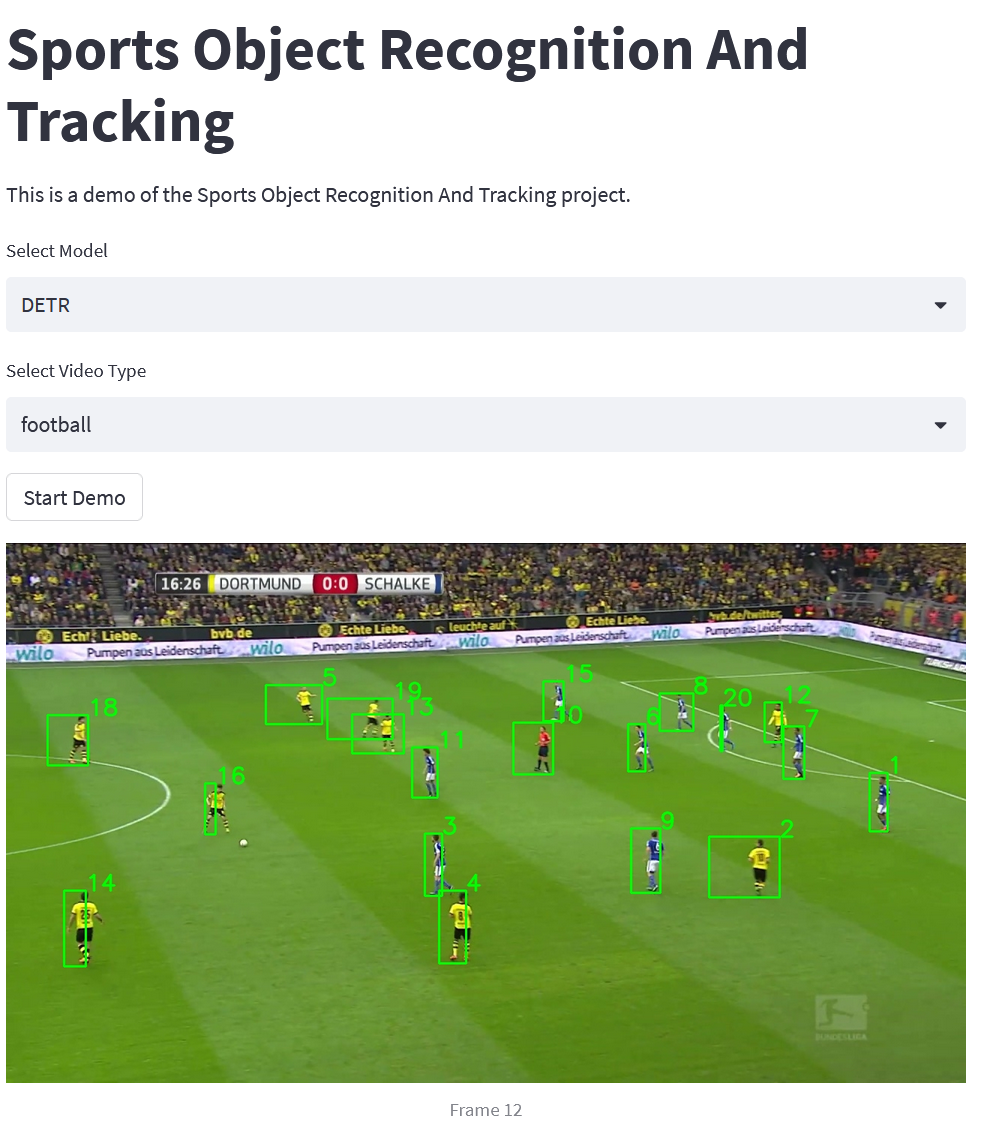
\includegraphics[width=\textwidth,height=13cm,keepaspectratio]{images/sport_demo.png}
    \caption{Demo website for viewing the results}
    \label{fig:sport_demo}
\end{figure}


\section{Challenges}
% Explain the challenges faced during the project
% Training time and computational resources
% Explain why the models were not finetuned

The main challenge faced during the project was the training time and computational resources.
The time required to train the models was very high.
And adding the time needed to do hyperparameter tuning made it even worse.
This made it difficult to achieve the desired results and come up with a new model.
Fine tuning was performed  on the DETR model for SportsMot dataset, but due to computational constraints good results were not achieved.

Reproducability is also a challenge in deep learning.
Trying to compare the results of different models is difficult as each needs a different environment and dataset loading pipeline.
So most time was spent on creating a framework that can be used to compare different models on the same dataset.

\section{Conclusion}
% TODO: Write conclusion
To conclude, the field of object detection and tracking has seen a lot of progress in the last few years.
With the introduction of SportsMot dataset, it has even more practical applications it can be used for.
Automatic annotation of sports videos can be used to generate highlights of the match.
With even better hardware they can be used in real-time to generate live highlights of the match.
This can be used to improve the experience of the viewers and also help the coaches in analyzing the performance of the players.

Accessing and setting up the dataset for benchmarking with a baseline model can be a challenging and time consuming task.
The framework proposed in this paper can be used to fasten this process.
With rapid improvements, this framework allows for easy integration of new models.

\section{Future Work}
% TODO: Write future work
For future work, the framework can be extended to include more models.
Currently only two models are implemented for object detection and one for object tracking.
More models can be added to the framework to allow for more comparisons.
The framework can also be extended to include more datasets.

Additionally, only pretrained models were utilized for this project.
Using the framework finetuning can be done in order to improve the performance of the models for the SportsMot dataset.
This will achieve better results and can be used to publish results for competition.
But this will require a lot of computational resources and time.

Another area of improvement is the hyperparameter tuning.
Currently the hyperparameters are set to the default values.
But with hyperparameter tuning the performance of the models can be improved.
Either by using a grid search or by using a more advanced method like Bayesian optimization.

% %
% ---- Bibliography ----
%
% BibTeX users should specify bibliography style 'splncs04'.
% References will then be sorted and formatted in the correct style.
%
\bibliographystyle{splncs04}
\bibliography{samplepaper}
% include references even if they are not cited in the text
\nocite{*}

\end{document}
